\documentclass[aps,prl,preprint,groupedaddress]{revtex4-1}
\usepackage{amsmath}
\usepackage{amssymb,amsfonts}
\usepackage[all,arc]{xy}
\usepackage{enumerate}
\usepackage{mathrsfs}

\usepackage{natbib}
\bibliographystyle{dinat}
\usepackage{graphicx}

\begin{document}
\title{SciNet: Promise and Pitfalls}

\author{Artem Bolshakov}
\affiliation{Cornell University}

\date{\today}

\begin{abstract}
In \cite{iten2020}, the authors present a very good interpolation technique, that can be used to identify some key variables that affect systems, as well as predict their behavior. Properly contextualized, with an understanding of the limitations of all neural methods (and this one specifically), this can be a powerful tool for an experimentalist or theorist. I hope to showcase this methods potential applications, pitfalls, and some mitigating techniques here, using several toy examples and a full-fledged analysis of the driven damped oscillator.
\end{abstract}

\maketitle

\section{Introduction}

The study of Neural Networks has numerous applications in the world today, both in practice, such as this translation software \cite{attention}, but also as a poweful tool for researchers in many different fields \cite{deeplabcut}. Despite this potential, however, many researchers in this field have a bad habit of promising even more and then not delivering. For instance, there is now a shortage of radiologists since Geoff Hinton warned back in 2016 that "if you're a radiologist, you're like a coyote who's already over the edge of the cliff but hasn't looked down yet." Furthermore, many truly fascinating advances are advertized far above their potential, so that even their impressive performance ends up being underwhelming. Another great example is Google Talks to Books; this system is capable of answering many questions if their answer is directly visible in a text from its corpus, reasonably competent at looking up reference material natural language. However, it was incorrectly advertised as "reading books," which it most certainly doesn't do: it is incapable of answering simple questions that require synthesizing even two or three pieces of information from different sources, or answering questions such as "where did Harry Potter meet Hermione" \cite{gmarticle}. This article, and the longer book (\cite{gmbook}) have a very good discussion of how modern AI falls short of the theories necessary to comprehend even basic children's books. I believe the same holds true for discovering physical theories.

Returning to \cite{iten2020}, then, I believe it falls into the last category, introducing an idea with impressive potential in physics, and then grossly exagerating that potential. The goal of this review is to showcase both the utility of this network, some of its failure modes (and why building on this foundation won't lead to physical laws), as well as advice on mitigating these pitfalls in practical applications.

\subsection{What SciNet Is and Isn't}

The article introduces a very powerful, general method for interpolating smooth, differentiable functions. Furthermore, using a clever reinterpretation of an old idea in ML - a Variational Autoencoder \cite{VAE} - the authors even expose some of the internal workings of their neural architecture, partially reducing the "black box" nature these models are notorious for. I belive this has a lot of potential in physics and other sciences; given some time, methods based on this framework might even become as useful and ubiquitous as local polynomial and Fourier approximations.

However, the authors are \textbf{certainly not} "Discovering Physical Concepts with Neural Networks," as the title claims. SciNet cannot be used outside of a larger, theoretical framework, using symbolic mathematics to describe physical laws. Nor is their agent "unbiased by prior knowledge," as the authors claim in the introduction; in fact, I will show how SciNet has specific, quantifiable biases towards smooth functions that are counterproductive in some cases. Not to mention, neural networks as a whole have biases towards simple functions, and without this bias they couldn't be useful fitting techniques \cite{simplicityBias}. The problem with these descriptions is not just that they are clickbait; it's that they are very likely to grossly mislead and misdirect new researchers, especially those who are more familiar with physics than they are with neural networks. If you don't understand the many, significant limitations of this approach, and naively throw difficult experimental data at it, you will only become incredibly frustrated, and possibly become disenchanted with the entire, fascinating field.

\subsection{How Should SciNet Be Used?} 

SciNet can be used in place of other interpolation techniques, such as polynomial interpolation - that is, on functions that are continuous, smooth without large jumps, on a restricted domain, and with a restricted range. A great example is $arcsin$, shown with its polynomial approximations (figure \ref{arcsin}). Note that the $arcsin$ nonlinearity appears in the transformation from geocentric to heliocentric coordinates, essential for the Solar System problem discussed in the original paper.

\begin{figure}[h]
   \centering
   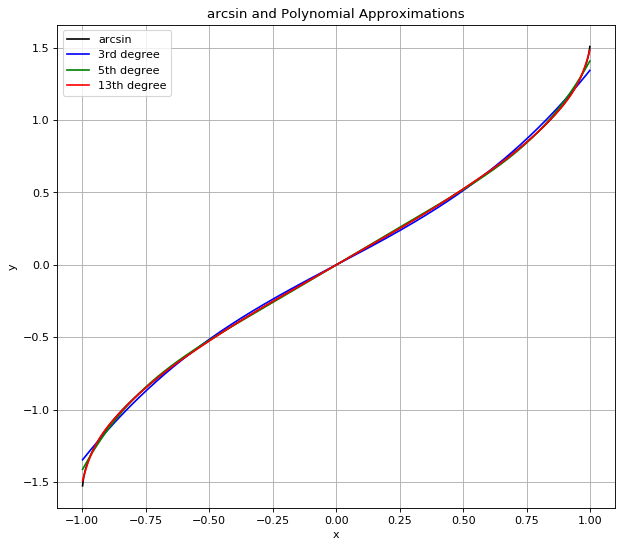
\includegraphics[width=0.8\textwidth]{mqfigs/arcsin.png}
   \caption{\label{arcsin} The $arcsin$ function, with several polynomials approximations. This function is a great candidate for all fitting techniques, since it has a bounded domain, bounded range, no discontinuities, and a small first derivative almost everywhere (except near $x = \pm 1$, where we seen the polynomial fits break away). This function is also part of the equation for computing heliocentric angles from geocentric angles, so its relatively easy for a neural network to learn that problem.}
\end{figure}

Unlike polynomials, it is particularly good with functionas that consume input many variables, but whose behavior is likely controlled by just a few values that can be derived from those functions. The behavior of the latent space might isolate those variables, or it might not, but there's certainly a chance that the behavior of the latent space can guide the scientist. SciNet can be used to make predictions in an area well covered by the training data, and possibly used in lieau of experiments (more in the Conclusion), but it should \emph{never} be used for extrapolation far from that domain, even if the underlying function is very simple, as we will see in section $3$.

There are many possible applications of this network, which I will suggest in the conclusion. There are also many cases in which we can use preprocessing in order to make difficult physical systems more tractable for SciNet, in case the researcher knows some aspects of the system he is studying; we'll discuss some of these in section $5$, and also in the conclusion.

This document is structured in the following way: in section $2$, I'll review the principles of neural networks and of SciNet in particular. In section $3$, I will discuss the problems and advantages of using neural networks for fitting functions in general, using two very simple ground truth functions. In section $4$, I will discuss the model problem of the driven, damped oscillator; in section $5$, we will see how the results showcasesome of the pitfalls of this method, as well as mitigating techniques. Finally, we will discuss these systems, general tips, and directions for future research in the conclusion.

\section{Neural Nets and VAEs}


Let's briefly review the underlying methods, before analyzing their potential.

\subsection{ Stochastic Gradient Descent}

Let's assume that we have input $x$ (of some dimension), and output $y$, also multidimensional. Let's say that $x$ is drawn from some distribution characterized by $P(x)$, while $y$ is given by $y \equiv F(x)$ in every $x$, $y$ pair. Generally, machine learning methods are equipped to handle situations in which the output has noise, so we must deal with a probability distribution $Q(y|x)$, but the deterministic case is enough for us.

At the core of any method that learns using stochastic gradient descent is a function $G$ with parameters $\theta$. In the case of neural nets specifically, $G$ is the network architecture while $\theta$ is the vector of weights and biases in the network. The goal of the learning procedure is to choose $\theta$ such that $G(x;\theta) \approx F(x)$ for most $x$ drawn from $P(x)$.

To do this, we will need a differentiable loss function $L$, such that, given any $x$ and $F(x)$, we can compute the loss $L(x) = L[F(x), G(x; \theta)]$, and, more iportandly, we can compute the gradient $\nabla_{\theta} L (x)$.

Ideally, we would choose $\theta$ that minimizes the expected value of the loss given the data distribution, $E(L)$, which we can do by following the gradient $\nabla_{\theta} E(L)$. However, we have no direct way of computing this value. Instead, we approximate it using a stochastic sample of $n$ values, $x_i$, following the gradient

$$ \nabla_{\theta} \left( \frac{1}{n}\Sigma_{i = 1}^n L[F(x_i), G(x_i; \theta)] \right) $$

It's worth noting that most modern applications (including the ones in later sections) do not naively multiply this gradient by a constant and then take a step. Instead, a more sophisticated gradient-based optimization algorithm is used, such as Adam, which has built-in protections against local minima and other inefficiencies. For more information, see the pytorch documentation, \cite{adamdocumentation}, or the original paper, \cite{adampaper}.

\subsection{ Neural Nets}

We'll focus only on neural nets composed out of fully connected layers, though there are many variations and improvements of this theme. A fully connected layer takes in input $x$, of dimension $n$, and produces output $y$ of dimension $m$. There are two important parts: a simple linear transformation, and a nonlinearity.

\subsubsection{ Aside on the nonlinearity}

The nonlinearity is a simple function, chosen ahead of time. Traditionally, the $sigmoid$ was used, defined by 

$$ sigmoid(x) = \frac{1}{1 + e^{-x}}$$

However, this function suffers from gradients close to $0$ on much of its domain, which complicates gradient descent. Most networks today use the rectified linear unit, or $ReLU$ nonlinearity, defined simply by 

$$ ReLU(x) = \max (x, 0) $$

This works well in most cases, and is easy to evaluate, but it isn't smooth (has a discontinuous first derivative). In order to avoid this problems, the authors of \cite{iten2020} chose to use a softened version, known as an exponential linear unit, or $ELU$, defined by 

$$ ELU(x) =  \left\{  \begin{align*} x & \text{ if } x > 0 \\ e^x - 1 &  \text{ otherwise.} \end{align*} \right.$$

All three are shown in figure \ref{allnonlin}.

\begin{figure}[h]
   \centering
   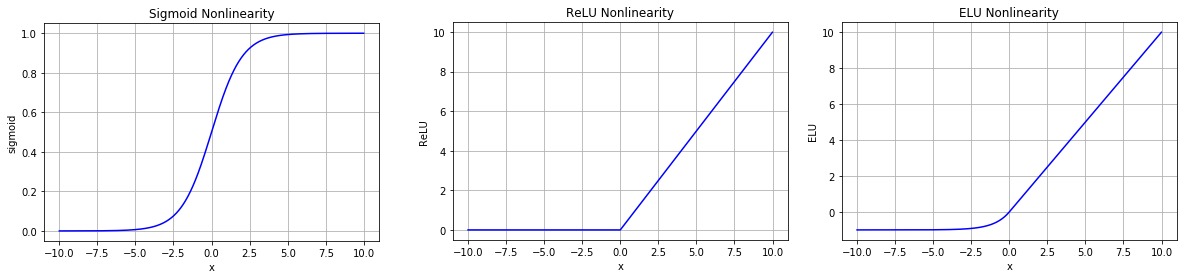
\includegraphics[width=1.0\textwidth]{mqfigs/nonlin_long.png}
   \caption{\label{allnonlin} Three nonlinearities used in neural networks; $sigmoid$, $ReLU$, and $ELU$, from left to right. Notice the different $y$ axis scales. The first two are more common, but the last was used in \cite{iten2020} and in my implementation of SciNet.}
\end{figure}

\subsubsection{ Putting it all together}

Assume we are using the $ReLU$ nonlinearity. Then, the output $y$ of our layer is defined by 

$$ y_i = ReLU\left( b_i + \Sigma_{i = 1}^n w_{ij}x_j \right), \text{ for all } 1 \le i \le m $$

The weights $w_{ij}$ and biases $b_i$ are the parameters $\theta$ of this layer. Each of the scalar variables $y_i$ is called a \emph{neuron}. Oftentimes, the value it takes on a particular computation is called an \emph{activation.}

Now, a neural network $G$ with layers $l_1, l_2, \ldots , l_k$ simply computes the output

$$ G(x; \theta) = l_k(l_{k -1} ( \ldots l_1(x))\ldots )$$

where $\theta$ is the vector of all the weights and biases of all of the layers. The gradient $\nabla_{\theta}$ is computed using an algorithm known as \emph{backpropagation,} essentially the chain rule. 

Note that the final layer $l_k$ often has a different nonlinearity than the others; for instance, one might use a $sigmoid$ instead of a $ReLU$ if the output must be between $0$ and $1$. In our case, the final layer has no nonlinearity at all, instead consisting of a simple linear transformation.

\begin{figure}[h]
   \centering
   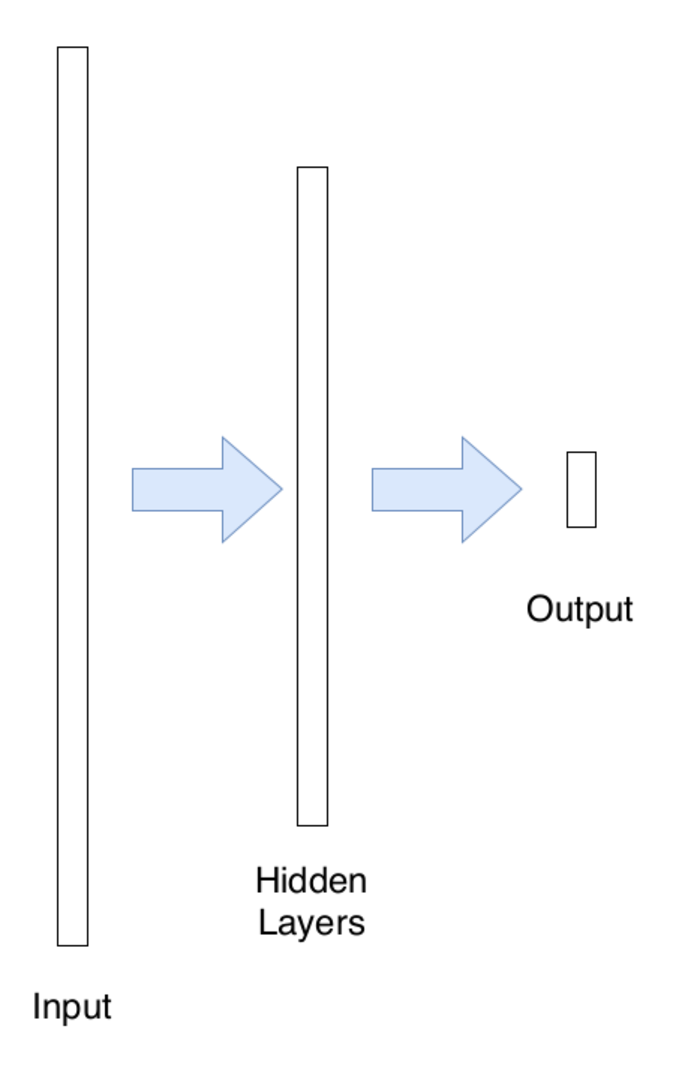
\includegraphics[width=0.4\textwidth]{mqfigs/Feedforward.pdf}
   \caption{\label{feedforward} A classic feedforward neural network, consuming high-dimensional input, passing through several hidden layers, and producing output, possibly low-dimensional classification information.}
\end{figure}

\subsection{ The Autoencoders, VAE and $\beta$VAE}

One particular architecture often studied in ML, known as an autoencoder, 
sets $y \equiv x$, for multidimensional $x$ and $y$ (note that this is not the case for SciNet). 
It would seem that learning the identity transofrmation would not be a problem for a neural architecture, 
but there is a complication: 
this system must learn to compress all of the complexity of the distribution $P(x)$ - 
which is usually a variable with many dimensions, such as an image - 
into a limited information bottleneck with just a few free parameters, $z$, 
as we can see in figure \ref{autoencoder}. 
The two parts of an autoencoder are the encoder $E$, such that $z = E(x)$, and the Decoder $D$, 
providing the reconstruction $y = D(z)$. 
The idea here is domain-specific compression, 
and possibly discovering "natural" axes along which $P(x)$ varies, 
possibly using the latent representation $z$ in some downstream model.

\begin{figure}[h]
   \centering
   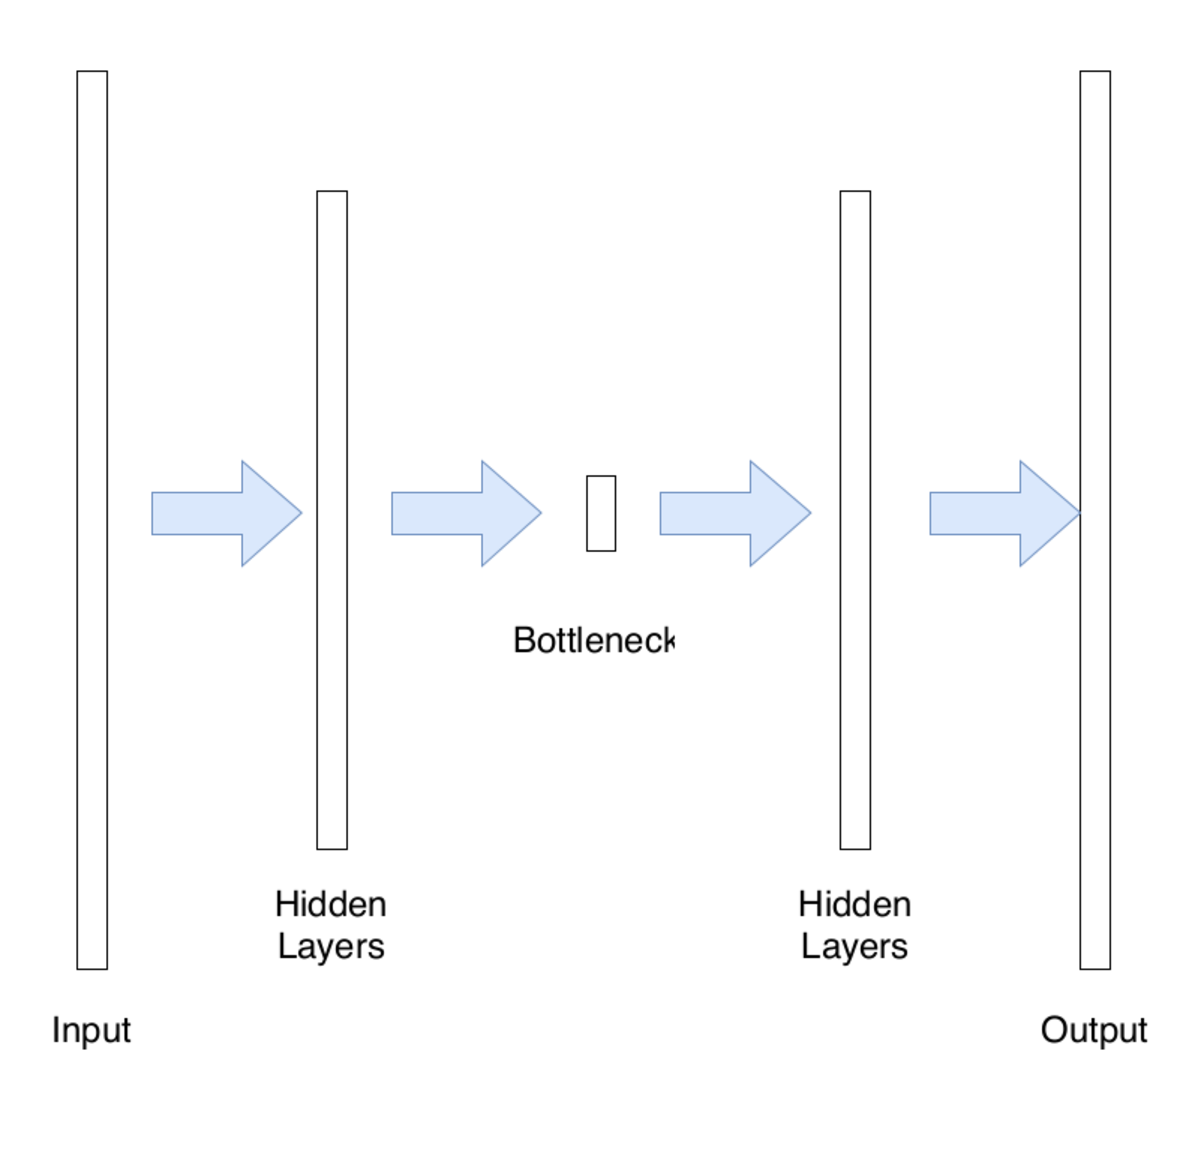
\includegraphics[width=0.8\textwidth]{mqfigs/Autoencoder.pdf}
   \caption{\label{autoencoder} An autoencoder, with an information bottleneck, trained to reproduce the input.}
\end{figure}
%[Figure with my autoencoder.]

The Variational Autoencoder (VAE, derived in \cite{VAE}), takes things a step further, 
fitting not just a deterministic encoding $z = E(x)$, but a conditional probability distribution, $P(z | x)$ (assumed to be a multivariate normal with a diagonal covariate matrix, with means $\mu_i(x)$ and standard deviations $\sigma_i(x)$). 
Furthermore, the VAE tries to encourage $z \sim h(z) = N(0, 1)$ after integrating out the effects of $x$; that way, it's easy to create fake $x$ by drawing random $z \sim N(0, 1)$ in the latent space, and then computing the decoding $D(z)$.

More information about VAEs and the derivation of their loss function can be found in \cite{VAE} or in appendix S4.1 of \cite{iten2020supplement}. To make a long story short, it achieves all of these objectives by minimizing the formula on page 14 (without the $\beta$ so far) in \cite{iten2020supplement}, 

$$ L = -\left[ \mathbb{E}_{z \sim p(z | x)} \log p(x | z) \right] + D_{KL}\left( p(z|x), h(z) \right) $$
which, under the assumption of Gaussian noise in the reconstruction, reduces to 

$$ \| y - x\| ^2 + 0.5\left( \Sigma_i \log(\sigma_i^2 ) - \mu_i^2 - \sigma_i^2 \right)$$

Now, while the above equation comes out directly from the derivation in \cite{VAE}, it's possible that the scale for the reconstruction loss or the KL divergence is wrong, so it makes sense to add a user-controlled parameter $\beta$ to establish the correct balance; and indeed, this was done in \cite{betaVAE}, producing the full equation

$$ \| y - x\| ^2 + 0.5\beta\left( \Sigma_i \log(\sigma_i^2 ) - \mu_i^2 - \sigma_i^2 \right)$$

Its worth noting that the original authors of \cite{betaVAE} used a parameter $\beta > 1$, in order to encourage their variables to be independent of each other, while the authors of \cite{iten2020} use a $\beta < 1$ (typically, around $1e-2$ or so), which actually makes this less likely. However, since they achieved their results with this setting, and since emphasizing the KL divergence more might break their setup, I'm going to use their setting, with $\beta = 0.01$.

Finally - drawing random samples $z$ from $P(z | x)$ is usually only done during training, whereas when we are evaluating the model's performance, we will set $z_i(x) = \mu_i(x)$ for all $x$, choosing the value with the highest likelihood.

\subsection{ Which Hidden Parameters are Used?}

Looking carefully at the loss above, we can notice that high values of $\mu_i$ are punished, while the optimal value for $\sigma_i$ is $1$. However, setting $\mu_i \equiv 0$ and $\sigma_i \equiv 1$ for all values of $x$ essentially turns the number $z_i$ into a random variable, useless for reconstruction. Therefore, given enough latent parameters, a trained network will use just enough $z_i$ for reconstruction, with $\mu_i$ varying significantly, while letting the other parameters $z_j$ be random, normal variables in order to reduce the KL term (with the decoder learning to ignore $z_j$).

It's easy to recognize which variables $z_i$ are used by the decoder by looking at a histogram of the values $\mu_i$, like the two in figure \ref{howchoose}, from a network called boring\_patch which I will describe later.

\begin{figure}[h]
   \centering
   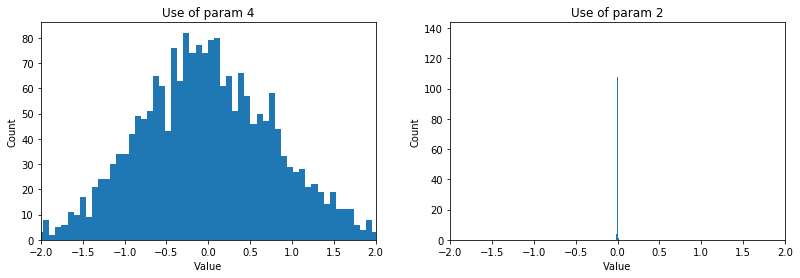
\includegraphics[width=0.8\textwidth]{mqfigs/sec2_paramhists.png}
   \caption{\label{howchoose} Two histograms for $\mu_i$, taken from latent variables of boring\_patch. The left parameter is used by the network, since this variable stores information differentiating the data; the right parameter is clearly not used.}
\end{figure}
%[TWO boring\_patch HISTOGRAMS]

If a variable is unused, all the values of $\mu_i$ will be near $0$, while if its used, the variables will be spread out, usually into something close to a normal distribution. The distinction is always very stark, so I didn't use any automatic cutoffs here. This is similar to what the authors of \cite{iten2020} describe; for an example, see Figure S3 from \cite{iten2020supplement} describing this procedure for their system modeling the conservation of angular momentum.

To finish, its worth mentioning that while the number of parameters used by a VAE or $\beta$VAE definitely suggests a value for the number of degrees of freedom in the problem (in the sense described in section S3 of \cite{iten2020supplement}), this is by no means a guarantee. Many different parameters can influence this, such as $\beta$, details about the size of the large and small efects, and even the total number of degrees of freedom available (that is, if a network with $n$ latent variables available learns to use $d < n$ degrees, a different network with $m > n$ latent variables might learn to use $f \not= d$ degrees, either more or fewer). We will see this in sections $4$ and $5$: while the ground truth physical problem definitely has exactly $2$ degrees of freedom, SciNet will both overestimate and underestimate this number in different experiemnts.

\subsection{SciNet}

SciNet uses a latent space with the same equations as above, but it is an example of supervised, not unsupervised learning. The $y$ values during training are not reconstructions, but rather data from some simulations. In addition, some implementations have question nodes in the latent space, variables controlled by the user in order to ask some question. All of this is summarized in their figure 1b, copied below in figure \ref{fig1b}, and described in more detail in \cite{iten2020}.

\begin{figure}[h]
   \centering
   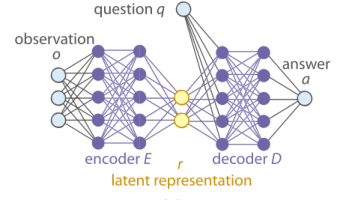
\includegraphics[width=0.8\textwidth]{mqfigs/their_Fig1b.pdf}
i   \caption{\label{fig1b} Figure 1b from \cite{iten2020}, showing the basic structure of SciNet: transform input into a latent representation using the same loss term as in a $\beta$VAE; augment this statespace with question node values; decode the entire structure to produce the output.}
\end{figure}
%[FIG 1b]

\section{Extrapolation}


One of the most impressive features of the laws of physics is how general they are, and how well they extrapolate far outside the original domain whence they were derived. Newton's Laws - even though we now know they are an imperfect approximation - extrapolate so well that the modern space industry still relies on them. The laws of physics as we understand them today apply so precisely to almost all the phenomena with which we can directly interact that experiments showcasing the limitations of modern theory require national or international megaprojects. In fact, it could be said that this capacity for extrapolation is \emph{the} feature that distinguishes physics from the other scientific disciplines; one would imagine that anything aiming to replace physical laws, as the authors of \cite{iten2020} suggest, would have the same feature.

However, neural networks have difficulty identifying even basic patterns and using them outside the training domain; overfitting is the rule. To see this, we will see how neural nets perform on the simple function

$$ y = x + 10 $$

We will use a one-dimensional $x$ and $y$, with $x \sim N(0, 1)$, and then evaluate performance for values of $x$ far from the origin.

\subsection{Theoretical Discussion}

Instead of testing the full SciNet here, I will focus on simple systems with just one hidden layer, with $8$ neurons in the hidden layer. This is not because SciNet wouldn't suffer from the same problems - I will try to show this by also including the results with $128$ hidden neurons - but because one layer is a simpler system, and we have the abilty to fully write out the effect of all parameters and understand all functions that can be described with such a system.

Specifically, for a system with $1$ dimensional input $x$, one dimensional output $y$, first layer weights and biases $w_{1, i} \text{ and } b_{1, i} 1 \le i \le 8$, second layer bias $b_2$, second layer weights $w_{2, i}$, and $ReLU$ nonlinearities, we can write

$$ y = b_2 + \Sigma_{i = 1}^8 w_{2, i} ReLU [ b_{1, i} + w_{1, i} x ]$$

In effect, we can fit any continuous, piecewise linear function with $8$ or fewer points where the slope changes. With $ELU$ nonlinearities, of course, we replace $ReLU$ with $ELU$ in the equiation, and the class of functions we can fit is slightly different, but the principle is similar.

Now, while an $ELU$ network can only approximate the function $f(x) = x + 10$ (at least, for $x$ drawn from the entire real line), clever choices for the weights and biases can express $f$ exactly in a $ReLU$ network. For example,

$$ x + 10 \equiv 10 + ReLU(x) - ReLU(-x) $$

However, there are also numerous ways for the functions to match only on a limited domain. For example, 

$$ x + 10 = ReLU(x + 10) $$

as long as $x \ge -10$ (which covers the entire training domain we are likely to encounter), but these functions quickly diverge for $x$ below this cutoff. 
Furthermore, there is nothing in the design of neural networks to encourage one solution over the other; the expectation is for the set of training points to cover all cases we are likely to see in the wild.

It's worth noting that this stands in sharp contrast to the tools typically used in physics, such as polynomial fits. Indeed, it's easy to prove that if we are performing a least squares fit with a polynomial of degree $k$, the ground truth function $f$ is a polynomial of degree $k$ or less (with no noise), and we have $k+1$ or more training data points, we are be guaranteed to recover $f$.

\subsection{Results}

Now that we understand why we have no reason for a neural network to extrapolate beyond the training domain, the results in Fig \ref{fail8} are easier to understand. I trained two networks, each with only one hidden layer of dimension $8$, and either ReLU or ELU nonlinearities. (Other paarameters: learning rate of $1e-4$, $2048$ new samples pulled every epoch for $50,000$ epochs, L2 loss).

\begin{figure}[h]
   \centering
   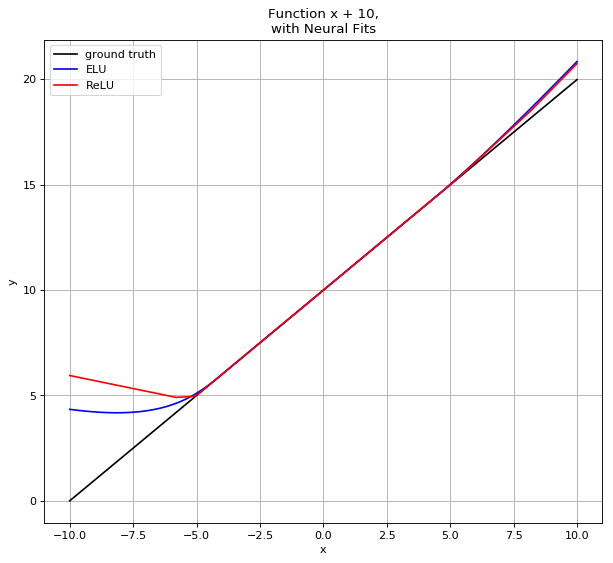
\includegraphics[width=0.8\textwidth]{mqfigs/8neuron_failure.png}
   \caption{\label{fail8} Ground truth function $y = x + 10$, with ReLU and ELU 8-neuron fits. The neural networks learn the function within the domain their training data is drawn from, but fail to extrapolate.}
\end{figure}
%[graph of failure, x in training range and outside it. FIG 1 LAYER.]

Adding more neurons in the hidden layer, or hidden layers, increases the flexibility of our model - we'll be able to fit piecewise linear functions with many more inflection points - but it does nothing to guarantee extrapolation.

\begin{figure}[h]
   \centering
   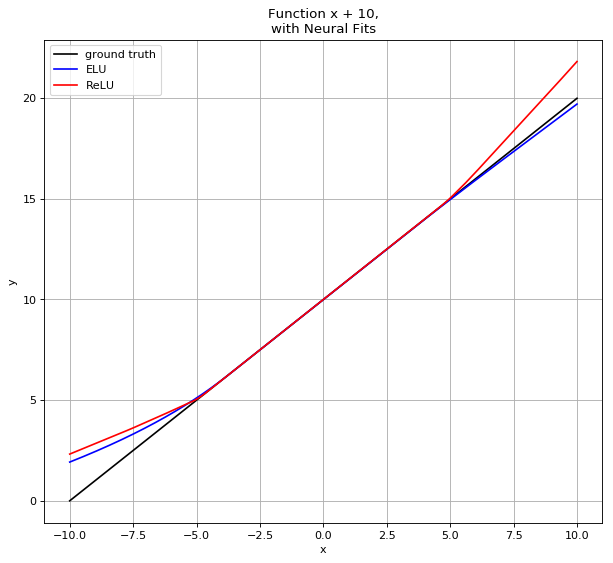
\includegraphics[width=0.8\textwidth]{mqfigs/128neuron_failure.png}
   \caption{\label{fail128} Ground truth function $y = x + 10$, with ReLU and ELU 128-neuron fits, showing the same behavior as the 8 neuron fits.}
\end{figure}
%[FIG WITH 128 NEURONS]

The same performance hurdles will hold true for more sophisticated systems, such as SciNet. There is nothing to guarantee that a system with good results on both the train and test set will still perform well outside of this set. Something as simple as increasing the amplitude of an oscillator by several factors of magnitude will break the predictive potential of the system.

We will see SciNet fail at far smaller extrapolations in Section $4$.

\subsection{Within the Training Distribution}

With such a strong bias away from functions that extrapolate, why use neural networks at all? Why not simply resort to more traditional techniques, such as polynomial fits?

Like every modeling tool, neural nets have their advantages and disadvantages. One of their strengths is their flexibility, and their ability to fit any function on a limited domain (this is known as the parametric limit, and it assumes a hidden layer with arbitrarily many inputs). 

Specifically, because all of the nonlinearities commonly used for neural nets are nearly linear or nearly constant on large segments of their domain, neural nets perform very good fits to functions that have different behavior in different parts of the relevant domain.

Perhaps the best function to showcase diferent behavior in different regions here is the discontinuous step function. Assume that $y = 10$ when $x > 0$ and $y = 0$ otherwise. With $x \sim N(0, 1)$, the graphs of trained ReLU and ELU neural nets (8 hidden layers, trained for 50,000 epochs) are in figure \ref{stepneural}.

\begin{figure}[h]
   \centering
   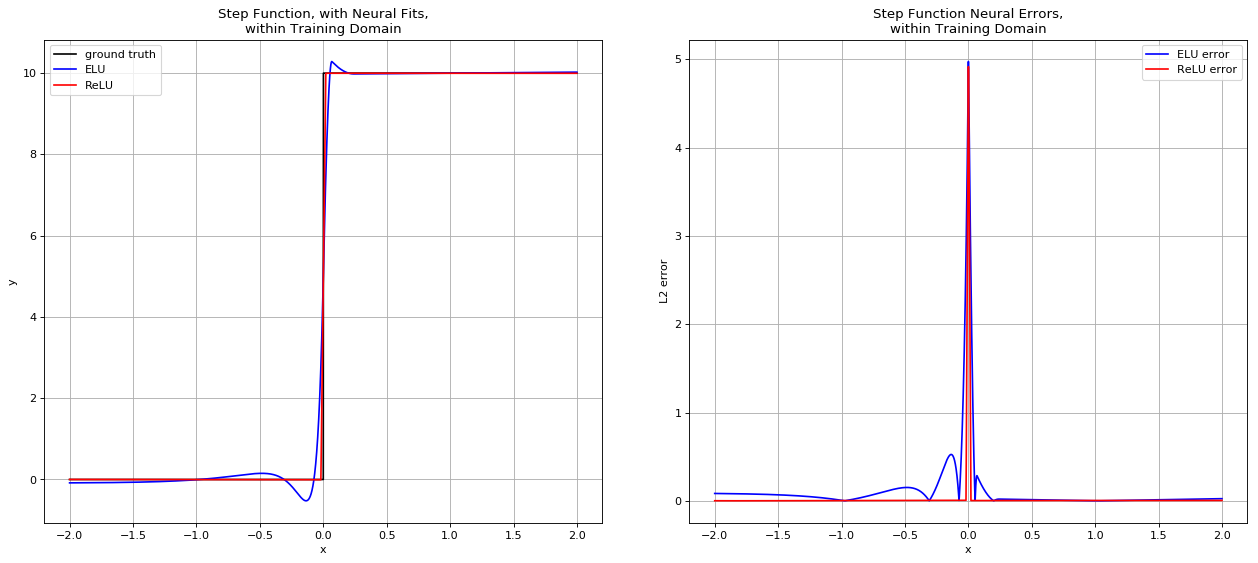
\includegraphics[width=1.0\textwidth]{mqfigs/step_neuralOnly.png}
   \caption{\label{stepneural} Neural fits to 10x the step function, and the error. Showing a section of the domain well-covered by training data (to be precise,$\mu \pm 2\sigma$).}
\end{figure}
%[Graph with ReLU and ELU approximation, as well as error.]

Away from the discontinuity, we see that the ReLU net matches the ground truth almost perfectly. The ELU net has small ringing effects, since it is limited to functions with a continuous first derivative, but these errors are also very small relative to the discontinuity.

However, if we take a polynomial of the same degree as the number of free parameters in these neural nets ($25$) and fit it to $204800$ $x$-$y$ pairs (the $xs$ were drawn from the unit normal), we get figure \ref{stepfull}. Changing the degree or the number of $x-y$ pairs within reasonable limits doesn't change the behavior much.

\begin{figure}[h]
   \centering
   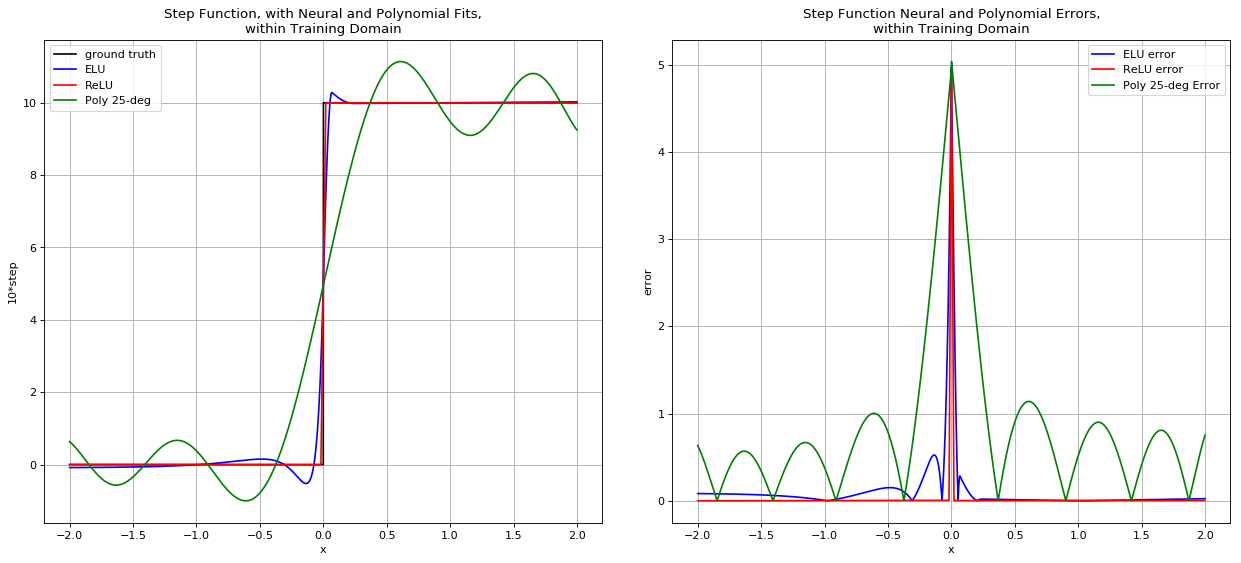
\includegraphics[width=1.0\textwidth]{mqfigs/step_full.png}
   \caption{\label{stepfull} Neural and polynomial fits to 10x the step function. The neural fits are much better.}
\end{figure}
%[GRAPH OF ABOVE, + POLYSTEP FAILURE]

If the ground truth is a polynomial, a polynomial fit will work very well, but if the underlying function is something different and you need to fit a patchwork of local behaviors, neural nets will do a far, far better job. If you have fewer ideas about the underlying system, fitting a neural net can direct you on the right path. SciNet can even identify some useful hidden variables which might make further investigation easier. However, if you want general rules that extrapolate well, further investigation is absolutely necessary; SciNet will not identify true "laws of physics" in any meaninful sense of the term.

\section{A Model Physical Problem}

It would be easy to break SciNet with an exotic, convolouted problem, such as mapping the precise shape of strange attractors or Lyapunov tongues, or predicting precise scaling factors and exponents near phase transitions. It would be even easier to show how poorly it extrapolates outside of its domain. However, none of this would highlight the problems with the approach described in \cite{iten2020} - after all, the authors never claimed that SciNet specificaly would replace the entire traditional field of Physics research, only that it is a first step capable of replacing theory in some limited examples. Throwing the most avant garde concepts at this fledgling method would not be fair.

Instead, I would need a simple problem, preferably one closely related to something the authors had studied. I would need something very common, a mechanism that explains many different behaviors and types of observational data, in many datasets and applications. Ideally, this would be a problem very well described and solved by conventional, even classical, methods, an old problem which would not strain any theorists. However, this problem still had to showcase all the drawbacks of the SciNet approach: poor extrapolation, sensitivity to the exact distribution of training data, difficulty working with assymptotes / discontinuities / poles, difficulty with handling regions with $y$ values with different orders of magnitude, and difficulty extracting any 'fundamental' latent space representations which tell us anything meaningful about the system.

I found everything I was looking for in the driven, damped oscillator, a complication on top of the damped oscillator the authors had studied. 

\subsection{ The Problem}

The full form of the driven, damped oscillator is described by the second order equation

$$ m\ddot{x} + 2\gamma \dot{x} + k x = A_o \cos \left( \omega t + \phi_0 \right) $$

However, most of the parameters only translate or scale the problem in space or time, changing the phase, amplitude, and fundamental frequency while preserving most features. Most interesting behaviors can be captured by the simplified problem

$$ \ddot{x} + 2\gamma \dot{x} + x = \cos (\omega t )$$

The response function of this system allows us to study the two most interesting effects - resonance and damping - without concerning ourselves with the phase of the stimulating signal or worrying about the space and time scales.

Focusing on the underdamped case, the steady-state solution to this equation is

$$
x(t) = A \cos (\omega t - \phi ) \\
\tan{\phi} = \frac{2\gamma \omega}{1 - \omega^2} \text{ , } 0 \le \phi \le \pi \\
A = \frac{1}{\sqrt{4\gamma^2\omega^2 + [1 - \omega^2]^2}}
$$

We could follow the treatment described on page 17 of \cite{iten2020supplement}, passing in a timeseries of previous values and seeing if SciNet can make predictions about future behavior; however, since we are working with the steady state solution only, that seems too easy; SciNet could easily just learn how to extract amplitude, frequency, and phase information from a cosine wave. Not to mention, even the results described in \cite{iten2020} for the damped pendulum essentially boil down to "teaching a neural network how to perform numerical differentiation and evaluating several periods of a cosine", and by now it shouldn't be too suprising that a neural network with several tens of thousands of free parameters can learn this trick.

Instead, I want to see if SciNet can handle a slightly more challenging regime where the experimentalist doesn't have access to the time series itself. This isn't that unrealistic; after all, driven oscillators describe a vast array of quantum and electrical system, and its often impossible to measure the very high-frequency oscillations themselves, while its perfectly possible to measure, say, the luminosity of a lightbulb driven by this electrical circuit, or even the phase lag between the driving and the stimulated signal; information that can be used to compute $A$ and $\phi$.

Therefore, given information about the damping coefficient $\gamma$ and the angular frequency $\omega$ of the driving signal - in a circuit experiment, these can be directly controlled using electrical components - I want to see if SciNet can produce a reasonable model that predicts the stimulated frequency $A$ and the phase difference $\phi$.

The graphs of $A$ and $\phi$ as a function of $\omega$ and $\gamma$ are in figure \ref{groundTruth}. 

\begin{figure}[h]
   \centering
   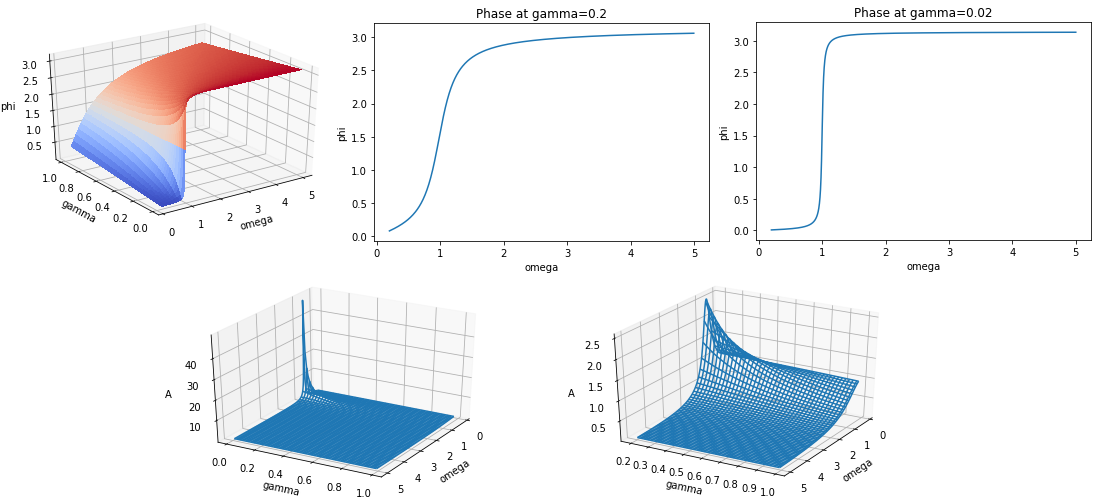
\includegraphics[width=1.0\textwidth]{mqfigs/phi_A_orig.png}
   \caption{\label{groundTruth} Graphs of $\phi$ (top) and $A$ (bottom) as a function of $\omega$ and $\gamma$. It might be easier to think of $\phi$ by taking slices of its dependence on stimulating frequency at different levels of damping (top center, right). $A$ has a discontinuous peak at $\omega =1, \gamma = 0$ (bottom left); other portions of $A(\omega, \gamma)$ are shown in the bottom right.}
\end{figure}
%[GRAPHS OF PHI AND A]

Notice the pole at $\gamma = 0, \omega = 1$; as we will see, the resonant spike in amplitude and the discontinuity in $\phi$ at this point (which has a complicated shape even without the huge errors produced by this variability in $A$), will be the main difficulties for SciNet.

We will also see whether changing to logspace - with both the domain and the range on a logscale, shown in figure \ref{logresults} - can improve the performance somewhat. Conceptually, this is to test how well SciNet can handle a training distribution that has a strange shape, but without huge, localized errors throwing off all of the results.

\begin{figure}[h]
   \centering
   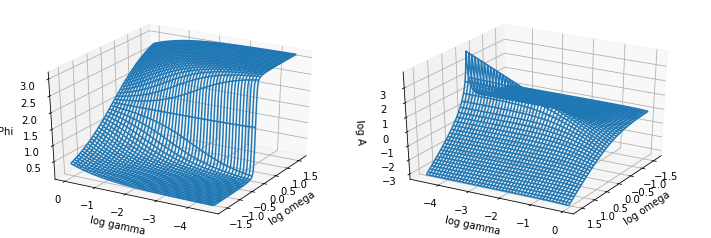
\includegraphics[width=0.8\textwidth]{mqfigs/phi_A_log.png}
   \caption{\label{logresults} Graphs of $\phi$ and $\log A$ as a function of $\log \omega$ and $\log gamma$. The functions maintain some interesting features, but we no longer need to contend with very large errors on any part of the domain.}
\end{figure}
%[GRAPHS OF LOGSPACE PHI AND A]

\subsection{ Technical Details of SciNet and Experiments}

This implementation of SciNet has $5$ latent variables; ideally, the network should learn to only use $2$, since there are $2$ degrees of freedom in both input and output. The training procedure consists of drawing $2048$ samples from a bivariate normal each epoch for $50000$ epochs, and using that data to take an optimization step (I didn't want to complicate the problem with concerns about overfitting, so I just assumed we had continuous access to the underlying distribution, or else a wealth of data we could sample from endlessly). I made sure to use the maximum dimensions that \cite{iten2020} had used for all hidden layers, with $[500, 100]$ in the encoder and $[100, 150]$ in the decoder. Like the original authors, I used the $ELU$ nonlinearity for functions with a continuous first derivative. I set $\beta = 0.01$; changing this might help with some of the problems in some, cases, but its a little unnatural to change it too much between trials, since SciNet is supposed to be a general technique. I always had two independent values in the output. 

A brief note on data generation: any datapoints with $\gamma < 1e-3$ were folded back into the realworld through a reflection over the line $\gamma = 1e-3$, to avoid particularly egregious values of $A$. This is particularly important for experiments concentrating on modeling ithe behavior near resonance. Values that left the underdamped regime with $\gamma > 1$ were also reflected back over that line. 

I ran $7$ experiments; $4$ in real-space, and $3$ in log-space ($\gamma$, $\omega$, and $A$ are replaced with $\ln \gamma$, $\ln \omega$, and $\ln A$, and training data is drawn from a normal distribution in logspace, while $\phi$ is passed in the same way it was before). Each was designed to capture a different facet of possible behavior; some more, some less successfully. Here are the means and standard deviations of these $7$ probability density distributions on the latent space:



%| Name | real / log | Mean of $ \omega $ | Mean of $ \gamma $ | Sigma of $ \omega $ | Sigma of $ \gamma $ |
%| ------ | ------- | ------- |
%| boring\_patch | real | 1.5 | 0.5 | 0.1 | 0.1 |
%| center\_very\_broad | real | 1.0 | 0.5 | 0.2 | 0.2 |
%| peak\_broad | real | 1.0 | 0.0 | 0.1 | 0.1 |
%| peak\_narrow | real | 1.0 | 0.0 | 0.01 | 0.01 |
%| logspace\_broad | log | $\ln (1.0)$ | $\ln (0.5)$ | 2.0 | 2.0 |
%| logspace\_near\_peak | log | $\ln (1.0)$ | $\ln (0.01)$ | 1.0 | 1.0 |
%| logspace\_near\_peak_narrow | log | $\ln (1.0)$ | $\ln (0.01)$ | 0.1 | 0.1 |
%
\begin{tabular}{ |p{5cm}||p{2cm}|p{2cm}|p{2cm}|p{2cm}|p{2cm}|  }
 \hline
 \multicolumn{6}{|c|}{Experiment Summary} \\
 \hline
 name& real / log & Mean of $\omega$&Mean of $\gamma$&Sigma of $\omega$&Sigma of $\gamma$\\
 \hline
 boring\_patch   & real &1.5&0.5&0.1&0.1\\
 center\_very\_broad   & real &1.0&0.5&0.2&0.2\\
 peak\_broad   & real &1.0&0.0&0.1&0.1\\
 peak\_narrow   & real &1.0&0.0&0.01&0.01\\
 logspace\_broad   & log &$\ln 1.0$&$\ln 0.5$&2.0&2.0\\
 logspace\_near\_peak   & log &$\ln 1.0$&$\ln 0.01$&1.0&1.0\\
 logspace\_near\_peak\_narrow   & log &$\ln 1.0$&$\ln 0.01$&0.1&0.1\\
 \hline
\end{tabular}

\section{Results}

SciNet managed with mixed success, closely matching behavior with some distributions of training points, but not others, suffering from extrapolation problems in all cases - the different networks certainly learned different global functions, even if they were all trained on the same underlying problem - and frequently using more than $2$ latent variables even though the problem has only $2$ input and output variables. Using a natural logarithm as preprocessing fixed some, but not all issues, clearly showing at least one way to mitigate the biases of this technique; we'll discuss others in the conclusion.

\subsection{ The Control: boring\_patch}

This is a patch far from resonance, where both $A$ and $\phi$ vary smoothly, as we can see in figure \ref{boringPhiA}. 

\begin{figure}[h]
   \centering
   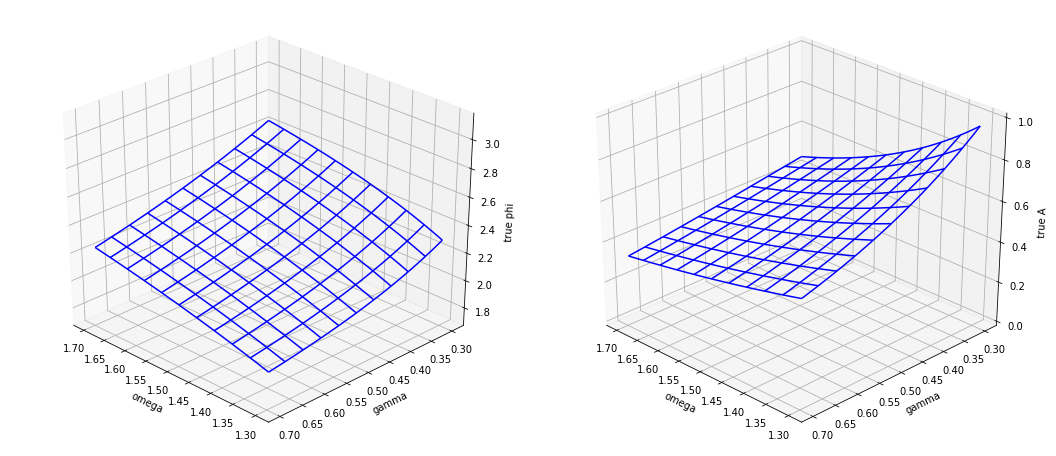
\includegraphics[width=0.8\textwidth]{mqfigs/boring_patch_true.png}
   \caption{\label{boringPhiA} Ground truth in the region well-covered by boring\_patch training data. $\phi$ left, $A$ right.}
\end{figure}
%[FIGURE A AND PHI IN BORING PATCH: NO FIT, $\pm$ 2 SIGMAS]

It serves as a control, to see whether SciNet is equipped for this problem at all. The result is: yes, it is, since the r.m.s. error is only $3.4$ percent of the range of $\phi$, while the r.m.s amplitude error is about $6.4$ percent. The performance within the training region showcases very well how similar the fit and the ground truth are, as we can see in \ref{boringModel}.

\begin{figure}[h]
  \centering
   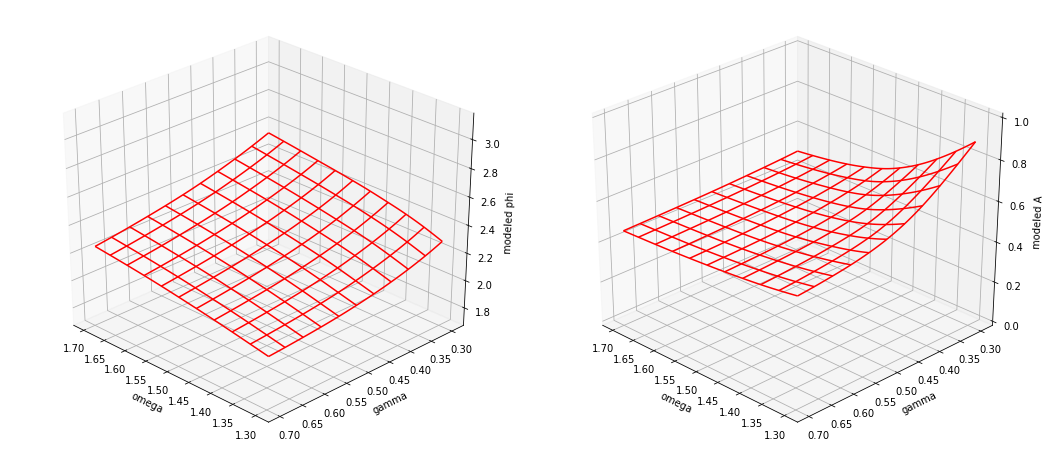
\includegraphics[width=0.8\textwidth]{mqfigs/boring_patch_model.png}
   \caption{\label{boringModel} The output of the boring\_patch model in the same region. $\phi$ left, $A$ right.}
\end{figure}
%[PHI AND A PLOTS OF BORING PATCH, MODEL ALONE.]

The latent space also follows expectations: 3 latent parameters are entirely unused, while parameters $3$ and $4$ are. The histograms of the $\mu$ values ofr these parameters aren't terribly far from normal distributions, as we can see in \ref{boringParamHists}

\begin{figure}[h]
   \centering
   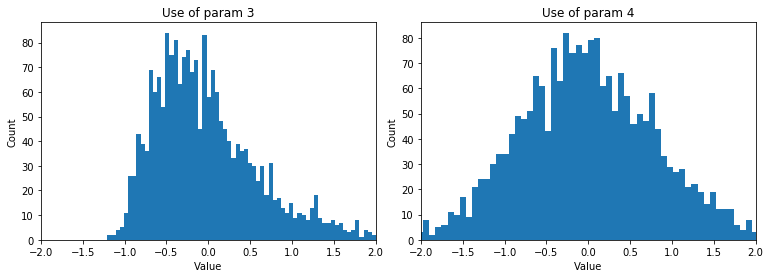
\includegraphics[width=0.8\textwidth]{mqfigs/boringpatch_param_hists.png}
   \caption{\label{boringParamHists} Histograms for boring\_patch parameters $3$ and $4$, showing that they are utilized by the network.}
\end{figure}
%[PARAMS 3 AND 4 HISTOGRAMS]

They don't seem to track any "natural" quantities (like $\omega \gamma$ or $1 - \gamma^2$), but they do track $A$ and $\phi$, respectively, almost exactly, (fig \ref{boringParamTracking}).

\begin{figure}[h]
   \centering
   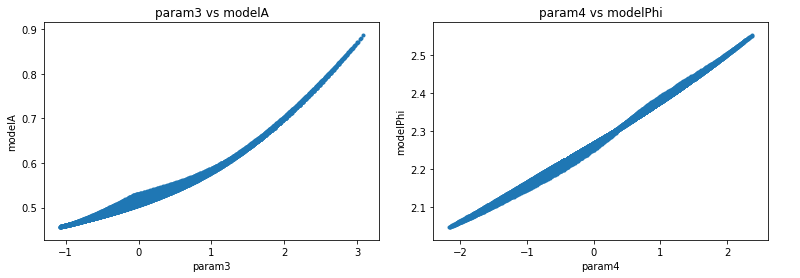
\includegraphics[width=0.8\textwidth]{mqfigs/boringpatch_param_tracking.png}
   \caption{\label{boringParamTracking} Graphs showing how the network uses the latent parameters to compute its estimate of $\phi$ and $A$. $\phi$ left, $A$ right.}
\end{figure}
%[FIGURE BORING PATCH PARAM TRACKING, END OF THAT IPYNB.]

Even the extrapolation seems somewhat sensible (fig \ref{boringExtrapolation}), if it doesn't capture the underlying ground truth.

\begin{figure}[h]
   \centering
   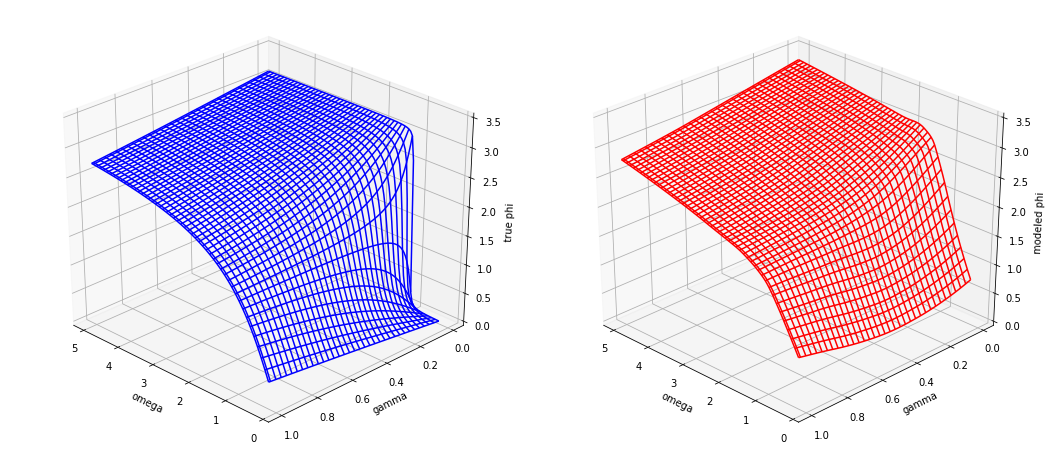
\includegraphics[width=0.8\textwidth]{mqfigs/boring_patch_extrapolation.png}
   \caption{\label{boringExtrapolation} Extrapolation of $\phi$ by boring\_patch. Ground truth left, model predictions right.}
\end{figure}
%[boringpatchextrapolation figure.]

\subsection{ Mixed Success: center\_very\_broad and peak\_broad}

These two experiments stretched the capabilities of SciNet without breaking them. The training data for center\_very\_broad was designed cover most of the interesting behavior in $\phi$ and $A$ while getting close to resonance, with some but few training points landing in that region, whereas peak\_broad covered was centered (close to) the resonant peak while also covering considerable ground arund it. We can see all of this in figures \ref{peakBroadSummary} and \ref{centerSummary}.

\begin{figure}[h]
   \centering
   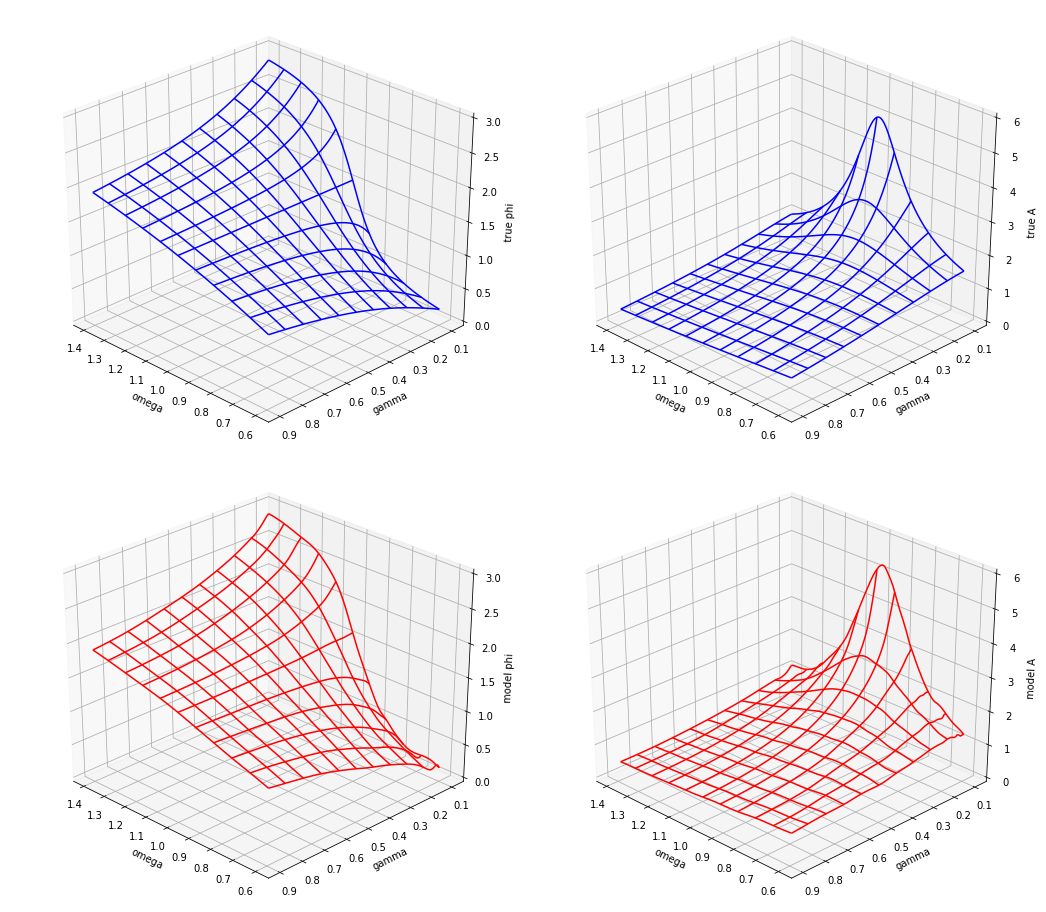
\includegraphics[width=0.8\textwidth]{mqfigs/center_very_broad_summary.png}
   \caption{\label{centerSummary} Ground truth (top, blue) and model (bottom, red), for both $\phi$ (left) and $A$ (right), for the model and domain of center\_very\_broad.}
\end{figure}
%[4 panel center\_very\_broad]

On average within the data distribution, the models from both center\_very\_broad and peak\_broad were within $2.8$ percent of the ground truth amplitude, which is impressive, since they had to match amplitudes that were both very large and rather small. In fact, the graph of model performance seems to be closer here than it is for boring\_patch (figures \ref{peakBroadSummary} and \ref{centerSummary}).

\begin{figure}[h]
   \centering
   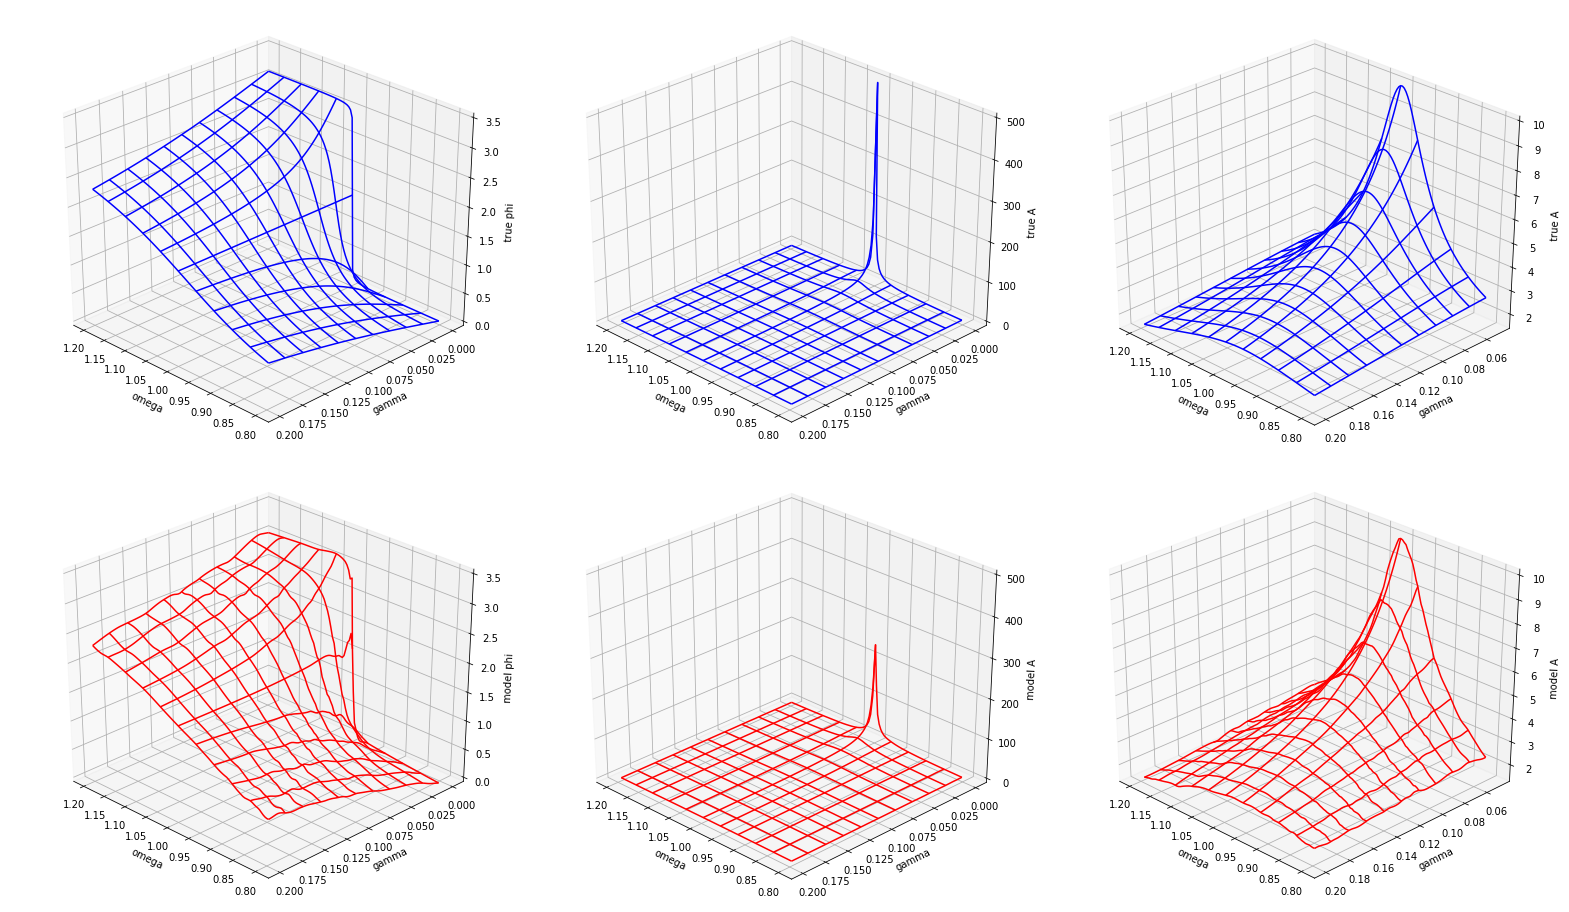
\includegraphics[width=1.0\textwidth]{mqfigs/peak_broad_summary.png}
   \caption{\label{peakBroadSummary} Ground truth (top, blue) and model (bottom, red), for both $\phi$ (left) and $A$ (center and right), for the model and domain of peak\_broad. Notice that the heights of the peaks are different (cutoff at $\gamma = 1e-3$), even though this region was within the training domain.}
\end{figure}
%[6 panel peak\_broad]

Once we look at the latent space distributions, we begin to understand why that might be: all $5$ parameters are used by both networks, and none of the latent $\mu$s seem to be distributed according to a unit normal. Nor do they seem to correspond as cleanly to $A$ or $\phi$. Fig \ref{centerParam3} shows the distribution and graph for parameter $3$ from center\_very\_broad, but they are all like that. It seems that the KL divergence was heavily dominated by the loss term during training.

\begin{figure}[h]
   \centering
   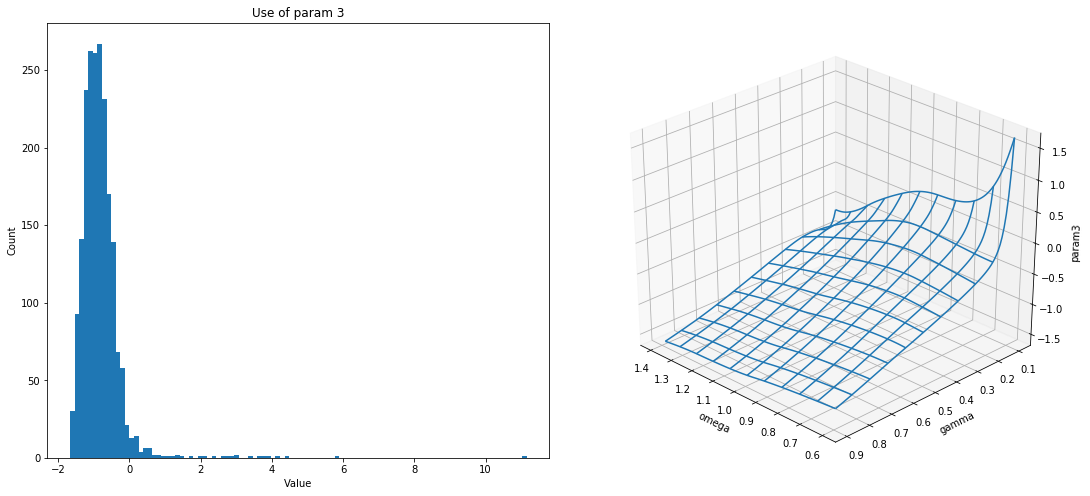
\includegraphics[width=0.8\textwidth]{mqfigs/center_very_broad_param3_full.png}
   \caption{\label{centerParam3} Parameter 3 histogram and graph for center\_very\_broad. It doesn't seem to correspond cleanly to either $A$ or $\phi$, or any simple function of the underlying variables.}
\end{figure}
%[SHOW HISTOGRAM AND GRAPH center\_very\_broad param3]

Finally, while we shouldn't expect good extrapolation from neural networks by this point, the behavior of the peak\_broad network far from its training distribution is interesting to look at (fig. \ref{peakBroadExtrapolation})

\begin{figure}[h]
   \centering
   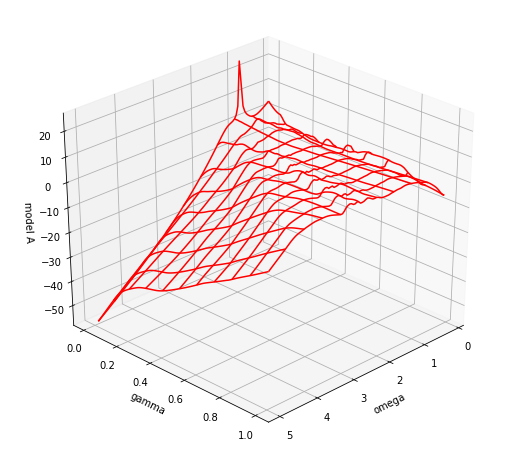
\includegraphics[width=0.6\textwidth]{mqfigs/peak_broad_extrapolation.png}
   \caption{\label{peakBroadExtrapolation} Extrapolatin by peak\_broad outside of its domain. Notice the $z$ scale.}
\end{figure}
%[EXTRAPOLATION PEAK\_BROAD MODEL ONLY, AMPLITUDE]

\subsection{ Outright Failure: peak\_narrow}

The purpose here was essentially the same as peak\_broad: to observe behavior on data trained immedeately around the discontinuity. The result is simple: the model simply wasn't trained. The learning curve clearly shows that it's gotten as good as it will get, yet fig. \ref{peakNarrowFailure} shows that the ground truth $\phi$ and modeled $\phi$ are nothing alike.

\begin{figure}[h]
   \centering
   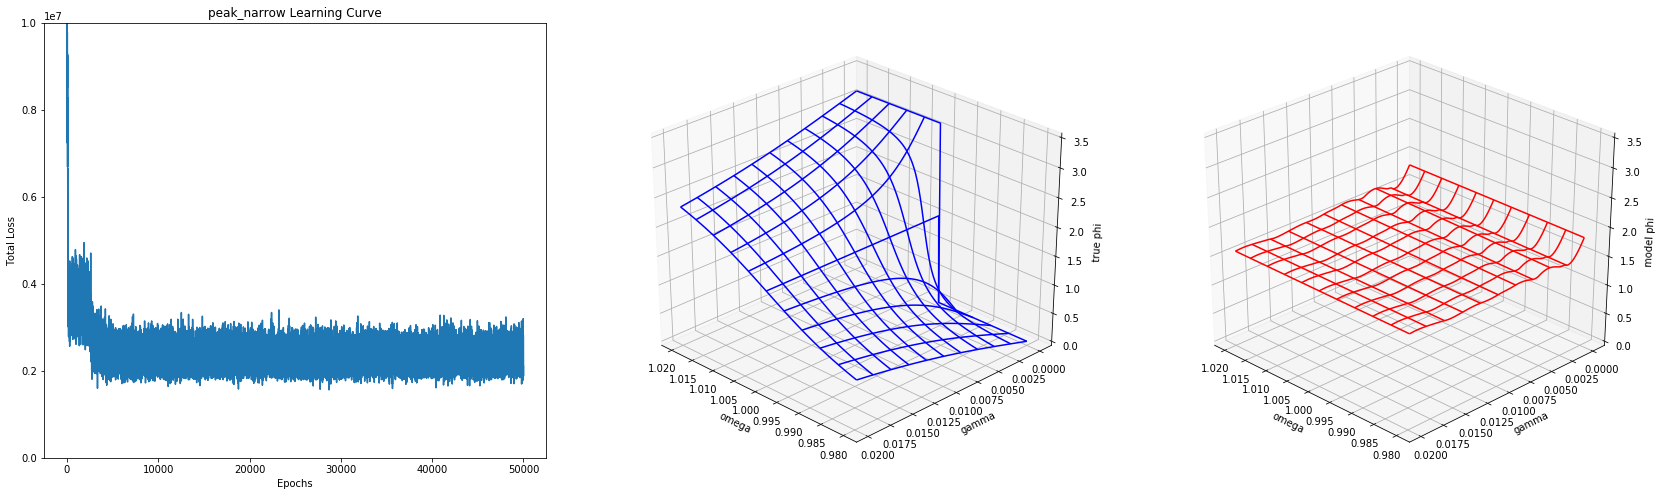
\includegraphics[width=1.0\textwidth]{mqfigs/peak_narrow_failure_long.png}
   \caption{\label{peakNarrowFailure} The learning curve (left), ground truth $\phi$ (center) and model-predicted $\phi$ (right) of peak\_narrow. It seems unlikely that further training would improve performance, and yet the ground truth function and the model output are very different from each other.}
\end{figure}
%[3 panel; Learning curve; ground truth $phi$ within training region; model phi within training region.]

However, it's not entirely fair to train the network on discontinuities only; what if we mitigate the difficult area by switch to logspace?

\subsection{ Mitigation: logspace\_broad and logspace\_near\_peak}

The idea was to train on a domain large enough to capture most of the interesting points, but in logspace, so that the sharp peak would ne more manageable. And it was; the average ampltude error divided by the amplitude range (in log coordinates) was around one part in one thousand, while the phase error was also less than $1$ percent. Plotting the training region, we see that the model captures practically all important features except for the asymptotically linear ridge, fig. \ref{4panelLogBroad}

\begin{figure}[h]
   \centering
   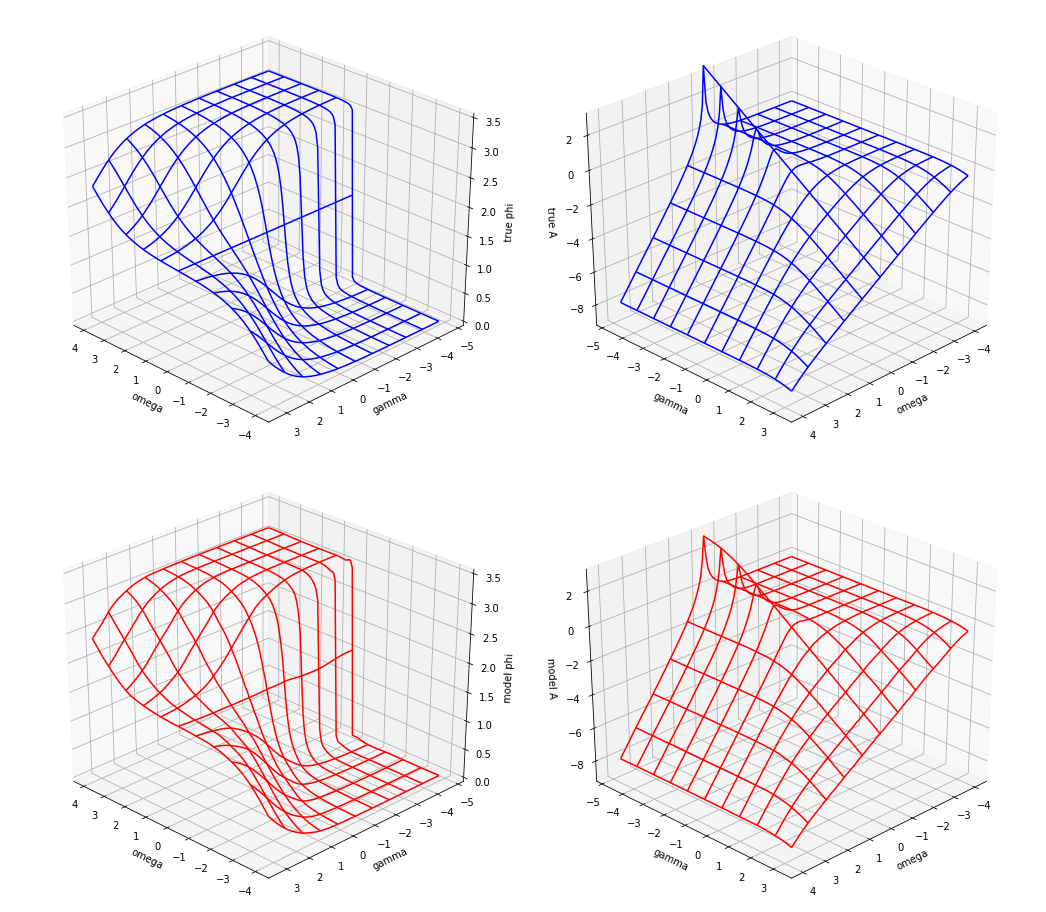
\includegraphics[width=0.8\textwidth]{mqfigs/logspace_broad.png}
   \caption{\label{4panelLogBroad} Ground truth (top, blue) and model (bottom, red), for both $\phi$ (left) and $\log A$ (right), for the model and domain of logspace\_broad.}
\end{figure}
%[4panelLogBroad: ground truth and model for phi and A]

The latent space behavior is also much better, with the network learning to use only $2$ latent parameters. It's also worth noting that the "ridge" does not extend under extrapolation (fig. \ref{badridge}), even though a theoretical description of the system would absolutely be able to fit that line.

\begin{figure}[h]
   \centering
   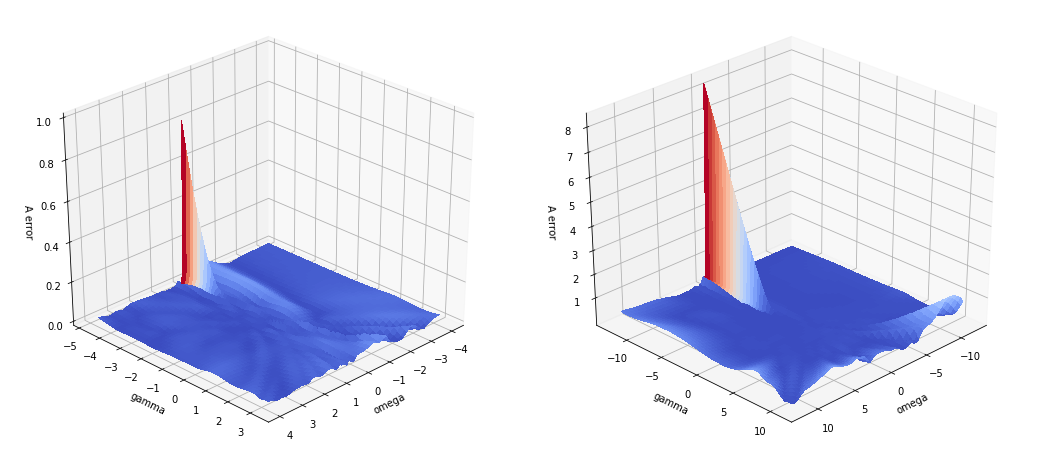
\includegraphics[width=0.8\textwidth]{mqfigs/logspace_broad_ridge_breakaway.png}
   \caption{\label{badridge} Graphs of logspace\_broad L2 error in $\log A$, both within the domain covered by training distribution (left), and further out (right). The ridge is not well captured by this model}
\end{figure}
%[Extrapolation, ridge breakeaway]

The model logspace\_near\_peak performs almost as well as logspace\_broad, with errors on the same scale, with the exception additional extrapolation mistake that none of the smoother portions of the $\phi$ function are matched, as in fig. \ref{logspaceNearPeakPhi}.

\begin{figure}[h]
   \centering
   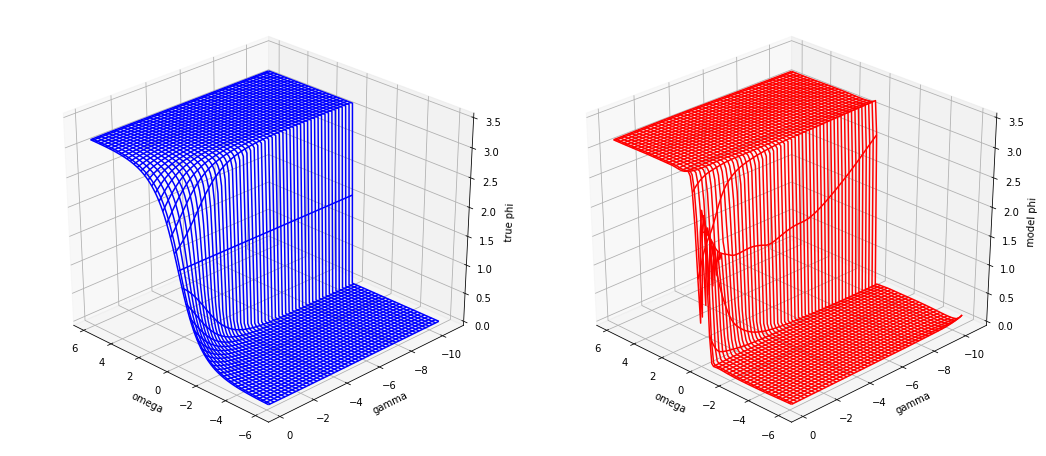
\includegraphics[width=0.8\textwidth]{mqfigs/logspace_near_peak_phi_extrapolation_6sig.png}
   \caption{\label{logspaceNearPeakPhi} Extrapolation mistake of logspace\_near\_peak, at $6\sigma$ away from the mean of the training distribution. The model does not predict any of the smoother portions of the $\phi$ function.}
\end{figure}
%[logspace\_near\_peak ground truth and model phi, separately, panels.]

\subsection{ Losing Small Effects: logspace\_near\_peak\_narrow}

Perhaps the most interesting failure mode - common to VAEs and SciNet - can be seen in logspace\_near\_peak\_narrow. Balancing reconstruction loss and KL divergence, the model ended up using just a single latent-space parameter, parameter $2$, which was almost proxy for $\omega$ depending very slightly on $\gamma$ (see fig. \ref{logspaceNearPeakNarrowParam2}), and did not pick up on the smaller $\gamma$-depednednt effects at all. This is most visible in a graph of the predicted and true $\ln A$, in fig. \ref{logspaceNearPeakNarrowA}. Errors were on the same scale as the other logspace models, however.

\begin{figure}[h]
   \centering
   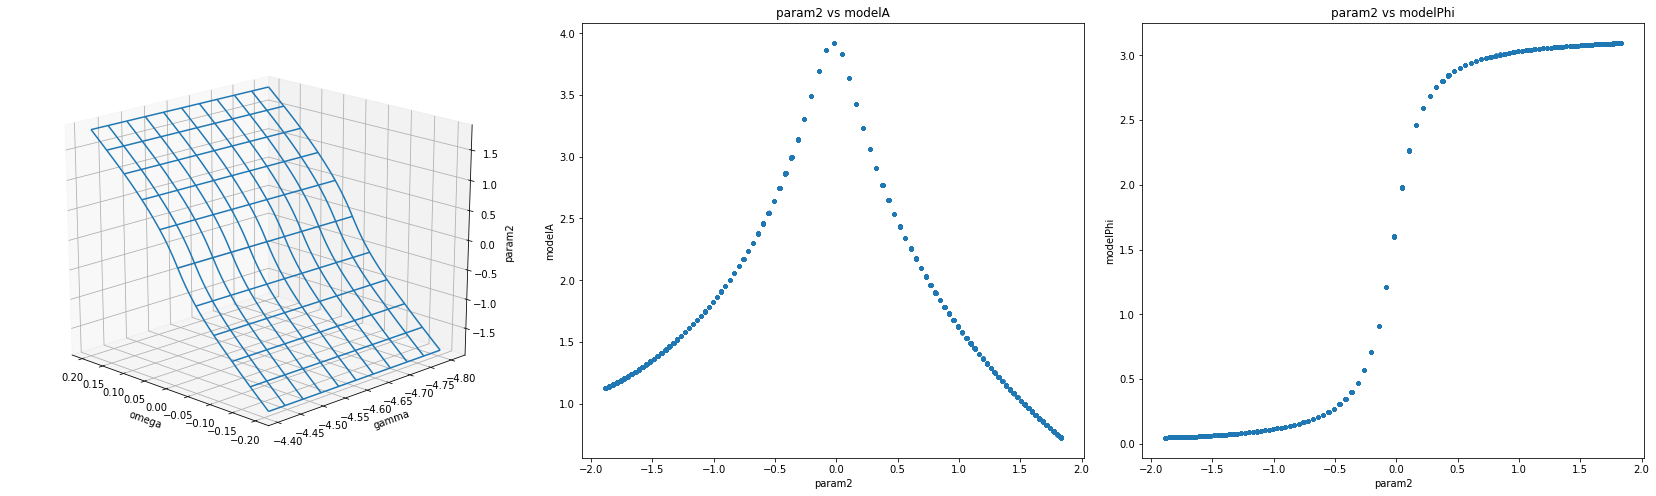
\includegraphics[width=1.0\textwidth]{mqfigs/logspace_near_peak_narrow_param2_long.png}
   \caption{\label{logspaceNearPeakNarrowParam2} The model logspace\_near\_peak learned to use just one parameter, parameter 2, to compute both its estimate of $A$ and $\phi$ (center and right, respectively). A graph of parameter $2$ - an almost linear function of $\log \omega$, with little $\log \gamma$ dependence, is shown on the left.}
\end{figure}
%[GRAPH OF NEAR\_PEAK PARAM2 IN TRAINING REGIONS]

\begin{figure}[h]
   \centering
   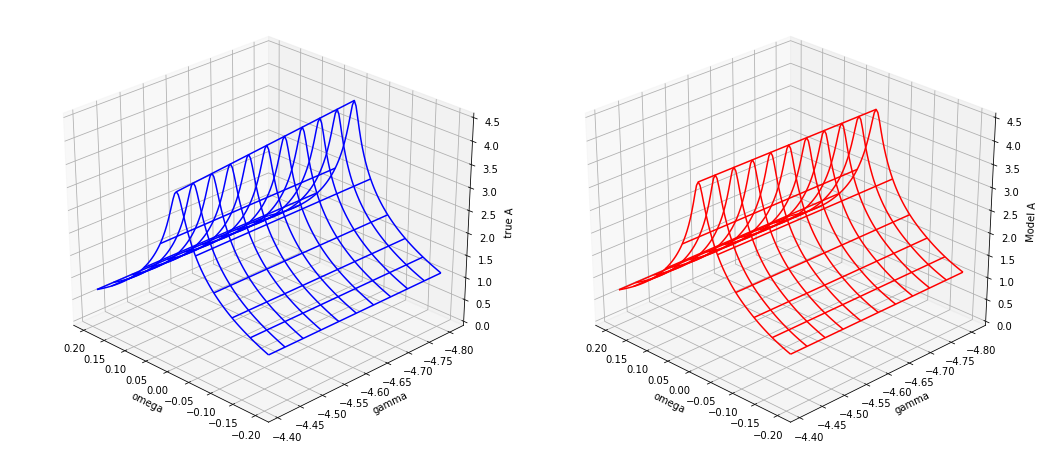
\includegraphics[width=1.0\textwidth]{mqfigs/logspace_near_peak_narrow_A.png}
   \caption{\label{logspaceNearPeakNarrowA} The problem with using only one of the latent parameters can be seen in a graph of $\log A$, where we see clearly that the ridge is not sloped at all in the model prediction, unlike the ground truth.}
\end{figure}
%[GRAPH OF GROUND TRUTH AND MODELED A]

\section{Conclusion}

It seems as if SciNet is a competent tool for performing nonlinear fits to data, and its latent space might provide some hints useful for further investigations (possibly extracting the quantity of degrees of freedom, if nothing else). Furthermore, some of the modifications discussed in the \cite{iten2020} - such as time dependence in the neural model of the solar system - might be very useful techniques for a physicist (or other scientist) to be familiar with. Finally, predictions by a well-trained version of SciNet might be very useful in an engineering application, where its difficult to make a very accurate model incorporating all the parameters, but collecting data on an existing implementation is quite easy. This is especially true if we are studying a problem where smaller effects can be safely ignored completely.

Using SciNet, the researcher needs to be very careful with the drawbacks of SciNet and neural networks in general, such as bad extrapolation and sensitivity to the details of the architectures, such as the size / number of hidden layers or the value of parameters like $\beta$.

After seeing all the possible failure modes, an experimentalist might be hesitant to use SciNet at all. The question arises; when should we use this method, and when should we use another one, like the sloppy model formalism derived by Sethna (basically, a technique for fitting a multivariate Gaussian with a vast array of different $\sigma$ values), or even perform a simple linear / polynomial fit as an approximation?

A simple case would be a dataset where other techniques have already failed. 
The system clearly isn't linear, polynomials make predictions which are probably artefacts,
and you would like to test something else. 
Additionally, the output function isn't any simple shape you recognize - simple interpolations seem to suggest a smooth, nonlinear function, but not anything simple you can describe elegantly theory. 
In such a case, SciNet might be a very worthwhile investment of time, as long as the output variables don't jump around too much.

Finally, if SciNet isn't performing well, but you have a good understanding of the data distribution, it might be a good idea to use preprocessing. The results from driven oscillators don't necessarily mean you can't use SciNet for spectrographic data, for instance; you just need to isolate the peak positions / heights, and pass those in instead of raw spectrograms. 

Overall, SciNet is a great, gentle introduction to many advanced applications within neural networks, and can be taught at the end of a good course on data science for physicists, graduate or undergraduate; or possibly, something based off of it could be a great project.

\clearpage
\bibliography{mertq}{}

\end{document}

